



\begin{figure}
\begin{subfigure}[b]{\textwidth}
\centering
\resizebox{0.55\textwidth}{!}{
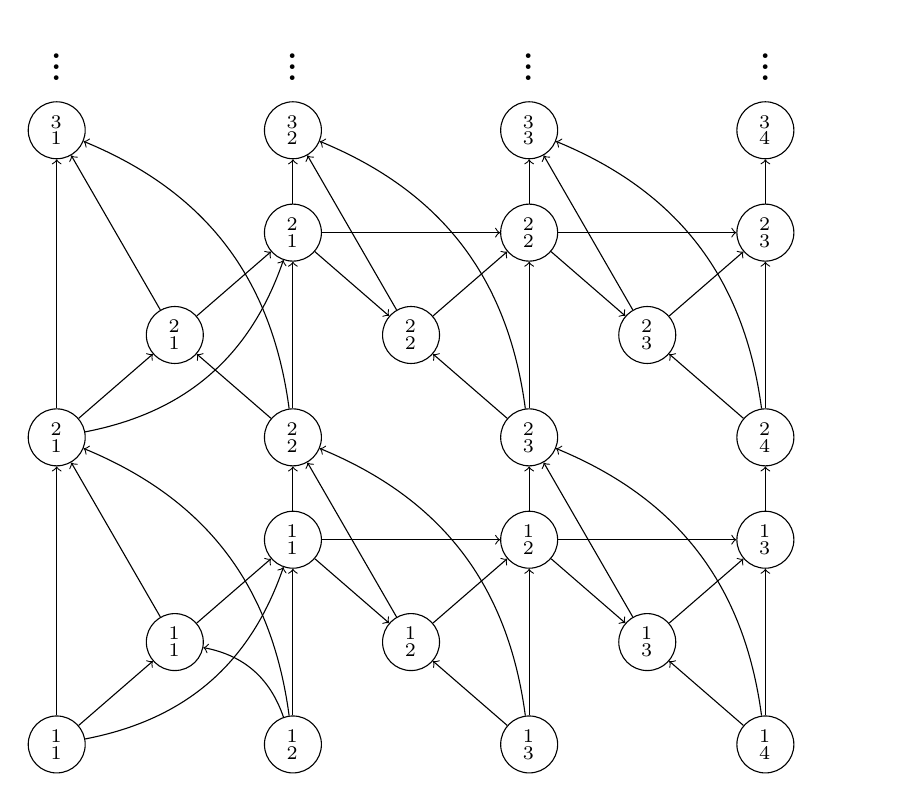
\begin{tikzpicture}

\def\xshift{3}
\def\yshift{1.3}

\node[circle,draw] (X11) at (0,0) {$\onevar^1_1$};
\node[circle,draw] (X12) at (\xshift, 0) {$\onevar^1_2$};
\node[circle,draw] (X13) at (\xshift*2, 0) {$\onevar^1_3$};
\node[circle,draw] (X14) at (\xshift*3, 0) {$\onevar^1_4$};
\node[] (X15) at (\xshift*3.5, 0) {$\huge\hdots$};

\node[circle,draw] (X21) at (0,\yshift*3) {$\onevar^2_1$};
\node[circle,draw] (X22) at (\xshift, \yshift*3) {$\onevar^2_2$};
\node[circle,draw] (X23) at (\xshift*2, \yshift*3) {$\onevar^2_3$};
\node[circle,draw] (X24) at (\xshift*3, \yshift*3) {$\onevar^2_4$};
\node[] (X25) at (\xshift*3.5, \yshift*3) {$\huge\hdots$};

\node[circle,draw] (X31) at (0,\yshift*6) {$\onevar^3_1$};
\node[circle,draw] (X32) at (\xshift, \yshift*6) {$\onevar^3_2$};
\node[circle,draw] (X33) at (\xshift*2, \yshift*6) {$\onevar^3_3$};
\node[circle,draw] (X34) at (\xshift*3, \yshift*6) {$\onevar^3_4$};
\node[] (X35) at (\xshift*3.5, \yshift*6) {$\huge\hdots$};


\node[] (d21) at (0,\yshift*6.7) {$\huge\vdots$};
\node[] (d22) at (\xshift, \yshift*6.7) {$\huge\vdots$};
\node[] (d23) at (\xshift*2, \yshift*6.7) {$\huge\vdots$};
\node[] (d24) at (\xshift*3, \yshift*6.7) {$\huge\vdots$};

\node[] (X25) at (\xshift*3.5, \yshift*2) {$\huge\hdots$};

\node[circle,draw] (B11) at (\xshift/2,\yshift) {$\onevarrr^1_1$};
\node[circle,draw] (B12) at (\xshift*3/2,\yshift) {$\onevarrr^1_2$};
\node[circle,draw] (B13) at (\xshift*5/2,\yshift) {$\onevarrr^1_3$};
\node[] () at (\xshift*7/2,\yshift) {$\huge\hdots$};

\node[circle,draw] (B21) at (\xshift/2,\yshift*4) {$\onevarrr^2_1$};
\node[circle,draw] (B22) at (\xshift*3/2,\yshift*4) {$\onevarrr^2_2$};
\node[circle,draw] (B23) at (\xshift*5/2,\yshift*4) {$\onevarrr^2_3$};
\node[] () at (\xshift*7/2,\yshift*4) {$\huge\hdots$};

\node[circle,draw] (Y11) at (\xshift,2*\yshift) {$\onevarr^1_1$};
\node[circle,draw] (Y12) at (\xshift*2,2*\yshift) {$\onevarr^1_2$};
\node[circle,draw] (Y13) at (\xshift*3,2*\yshift) {$\onevarr^1_3$};
\node[] () at (\xshift*7/2,\yshift*2) {$\huge\hdots$};

\node[circle,draw] (Y21) at (\xshift,5*\yshift) {$\onevarr^2_1$};
\node[circle,draw] (Y22) at (\xshift*2,5*\yshift) {$\onevarr^2_2$};
\node[circle,draw] (Y23) at (\xshift*3,5*\yshift) {$\onevarr^2_3$};
\node[] () at (\xshift*7/2,\yshift*5) {$\huge\hdots$};

\draw[->] (X11) to (B11);
\draw[->, bend right] (X12) to (B11);

\draw[->] (X11) to (X21);
\draw[->, bend right] (X12) to (X21);
\draw[->] (B11) to (X21);

\draw[->, bend right] (X11) to (Y11);
\draw[->] (X12) to (Y11);
\draw[->] (B11) to (Y11);

\draw[->] (Y11) to (B12);
\draw[->] (X13) to (B12);

\draw[->] (Y11) to (X22);
\draw[->] (B12) to (X22);
\draw[->, bend right] (X13) to (X22);

\draw[->] (Y11) to (Y12);
\draw[->] (X13) to (Y12);
\draw[->] (B12) to (Y12);

\draw[->] (Y12) to (Y13);
\draw[->] (X14) to (Y13);
\draw[->] (B13) to (Y13);

\draw[->] (Y12) to (B13);
\draw[->] (X14) to (B13);

\draw[->] (Y12) to (X23);
\draw[->] (B13) to (X23);
\draw[->, bend right] (X14) to (X23);

\draw[->] (Y13) to (X24);

\draw[->] (X21) to (B21);
\draw[->] (X22) to (B21);

\draw[->] (X21) to (X31);
\draw[->, bend right] (X22) to (X31);
\draw[->] (B21) to (X31);

\draw[->, bend right] (X21) to (Y21);
\draw[->] (X22) to (Y21);
\draw[->] (B21) to (Y21);

\draw[->] (Y21) to (B22);
\draw[->] (X23) to (B22);

\draw[->] (Y21) to (X32);
\draw[->] (B22) to (X32);
\draw[->, bend right] (X23) to (X32);

\draw[->] (Y21) to (Y22);
\draw[->] (X23) to (Y22);
\draw[->] (B22) to (Y22);

\draw[->] (Y22) to (Y23);
\draw[->] (X24) to (Y23);
\draw[->] (B23) to (Y23);

\draw[->] (Y22) to (B23);
\draw[->] (X24) to (B23);

\draw[->] (Y22) to (X33);
\draw[->] (B23) to (X33);
\draw[->, bend right] (X24) to (X33);

\draw[->] (Y23) to (X34);

\end{tikzpicture}}
\caption{A causal model that represents the bubble sort algorithm.}
\label{fig:bub1}
\end{subfigure}

\begin{subfigure}[b]{\textwidth}
\centering
\resizebox{0.55\textwidth}{!}{
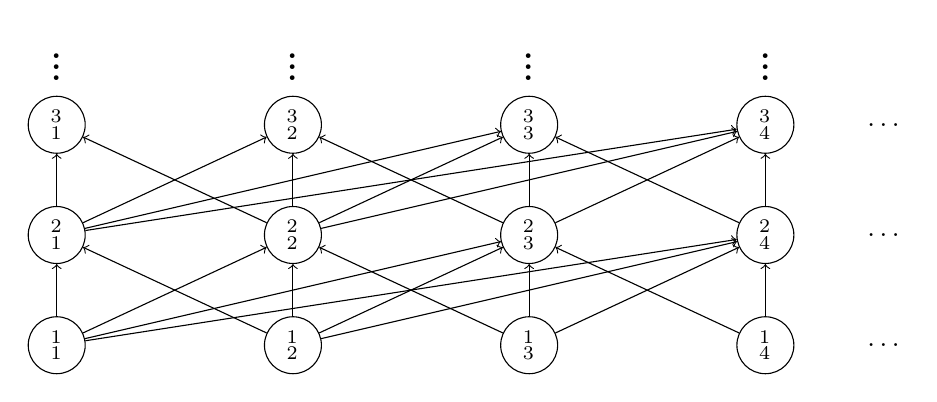
\begin{tikzpicture}
\def\xshift{3}
\def\yshift{1.4}

\node[circle,draw] (X11) at (0,0) {$\onevar^1_1$};
\node[circle,draw] (X12) at (\xshift, 0) {$\onevar^1_2$};
\node[circle,draw] (X13) at (\xshift*2, 0) {$\onevar^1_3$};
\node[circle,draw] (X14) at (\xshift*3, 0) {$\onevar^1_4$};
\node[] (X15) at (\xshift*3.5, 0) {$\huge\dots$};

\node[circle,draw] (X21) at (0,\yshift*1) {$\onevar^2_1$};
\node[circle,draw] (X22) at (\xshift, \yshift*1) {$\onevar^2_2$};
\node[circle,draw] (X23) at (\xshift*2, \yshift*1) {$\onevar^2_3$};
\node[circle,draw] (X24) at (\xshift*3, \yshift*1) {$\onevar^2_4$};
\node[] (X25) at (\xshift*3.5, \yshift*1) {$\huge\dots$};

\node[circle,draw] (X31) at (0,\yshift*2) {$\onevar^3_1$};
\node[circle,draw] (X32) at (\xshift, \yshift*2) {$\onevar^3_2$};
\node[circle,draw] (X33) at (\xshift*2, \yshift*2) {$\onevar^3_3$};
\node[circle,draw] (X34) at (\xshift*3, \yshift*2) {$\onevar^3_4$};
\node[] (X35) at (\xshift*3.5, \yshift*2) {$\huge\dots$};

\node[] (d21) at (0,\yshift*2.6) {$\huge\vdots$};
\node[] (d22) at (\xshift, \yshift*2.6) {$\huge\vdots$};
\node[] (d23) at (\xshift*2, \yshift*2.6) {$\huge\vdots$};
\node[] (d24) at (\xshift*3, \yshift*2.6) {$\huge\vdots$};

\draw[->] (X11) to (X24);
\draw[->] (X12) to (X24);
\draw[->] (X13) to (X24);
\draw[->] (X14) to (X24);

\draw[->] (X21) to (X34);
\draw[->] (X22) to (X34);
\draw[->] (X23) to (X34);
\draw[->] (X24) to (X34);

\draw[->] (X11) to (X23);
\draw[->] (X12) to (X23);
\draw[->] (X13) to (X23);
\draw[->] (X14) to (X23);

\draw[->] (X21) to (X33);
\draw[->] (X22) to (X33);
\draw[->] (X23) to (X33);
\draw[->] (X24) to (X33);

\draw[->] (X11) to (X22);
\draw[->] (X12) to (X22);
\draw[->] (X13) to (X22);

\draw[->] (X21) to (X32);
\draw[->] (X22) to (X32);
\draw[->] (X23) to (X32);

\draw[->] (X11) to (X21);
\draw[->] (X12) to (X21);

\draw[->] (X21) to (X31);
\draw[->] (X22) to (X31);
\end{tikzpicture}
}
\caption{The causal model from Figure~\ref{fig:bub1} with the variables $\onevarr^i_j$ and $\onevarrr^i_j$ marginalized.}
\label{fig:bub2}
\end{subfigure}
     
\begin{subfigure}[b]{\textwidth}
\centering
\resizebox{0.55\textwidth}{!}{
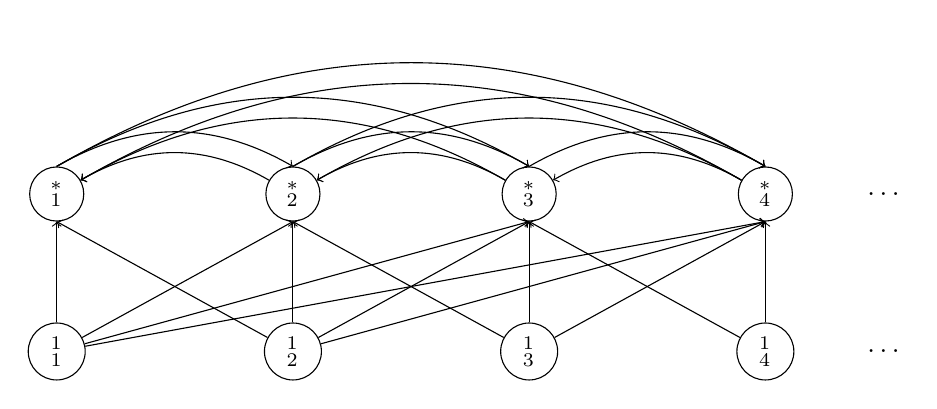
\begin{tikzpicture}
\def\xshift{3}
\def\yshift{1.4}

\node[circle,draw] (X11) at (0,0) {$\onevar^*_1$};
\node[circle,draw] (X12) at (\xshift, 0) {$\onevar^*_2$};
\node[circle,draw] (X13) at (\xshift*2, 0) {$\onevar^*_3$};
\node[circle,draw] (X14) at (\xshift*3, 0) {$\onevar^*_4$};
\node[] (X15) at (\xshift*3.5, 0) {$\huge\dots$};

\node[circle,draw] (X01) at (0,-2) {$\onevar^1_1$};
\node[circle,draw] (X02) at (\xshift, -2) {$\onevar_2^1$};
\node[circle,draw] (X03) at (\xshift*2,-2) {$\onevar_3^1$};
\node[circle,draw] (X04) at (\xshift*3,-2) {$\onevar_4^1$};
\node[] (X05) at (\xshift*3.5, -2) {$\huge\dots$};

\draw[->, bend left] (X11.north) to (X12.north);
\draw[->, bend left] (X11.north) to (X13.north);
\draw[->, bend left] (X11.north) to (X14.north);

\draw[->, bend right] (X12) to (X11);
\draw[->, bend left] (X12.north) to (X13.north);
\draw[->, bend left] (X12.north) to (X14.north);

\draw[->, bend right] (X13) to (X12);
\draw[->, bend left] (X13.north) to (X14.north);
\draw[->, bend right] (X13) to (X11);

\draw[->, bend right] (X14) to (X13);
\draw[->, bend right] (X14) to (X12);
\draw[->, bend right] (X14) to (X11);

\draw[->] (X01) to (X11.south);
\draw[->] (X01) to (X12.south);
\draw[->] (X01) to (X13.south);
\draw[->] (X01) to (X14.south);

\draw[->] (X02) to (X11.south);
\draw[->] (X02) to (X12.south);
\draw[->] (X02) to (X13.south);
\draw[->] (X02) to (X14.south);

\draw[->] (X03) to (X12.south);
\draw[->] (X03) to (X13.south);
\draw[->] (X03) to (X14.south);

\draw[->] (X04) to (X13.south);
\draw[->] (X04) to (X14.south);


\end{tikzpicture}}
\caption{The causal model from Figure~\ref{fig:bub2} with the variables $\onevar^2_i, \onevar^3_i, \dots$ merged for all $i>0$. The values of these new variables contain the full history of the algorithm, e.g., the value of $\onevar^*_1$ a sequence containing the first element in the list after each bubbling iteration.}
\label{fig:bub3}
\end{subfigure}
\begin{subfigure}[b]{\textwidth}
\centering
\resizebox{0.55\textwidth}{!}{
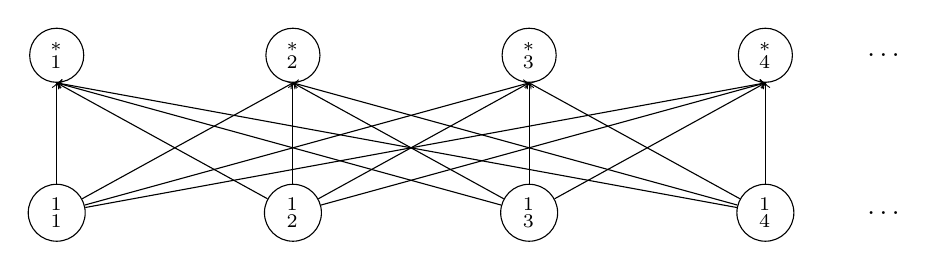
\begin{tikzpicture}
\def\xshift{3}
\def\yshift{1.4}

\node[circle,draw] (X11) at (0,0) {$\onevar^*_1$};
\node[circle,draw] (X12) at (\xshift, 0) {$\onevar^*_2$};
\node[circle,draw] (X13) at (\xshift*2, 0) {$\onevar^*_3$};
\node[circle,draw] (X14) at (\xshift*3, 0) {$\onevar^*_4$};
\node[] (X15) at (\xshift*3.5, 0) {$\huge\dots$};

\node[circle,draw] (X01) at (0,-2) {$\onevar^1_1$};
\node[circle,draw] (X02) at (\xshift, -2) {$\onevar_2^1$};
\node[circle,draw] (X03) at (\xshift*2,-2) {$\onevar_3^1$};
\node[circle,draw] (X04) at (\xshift*3,-2) {$\onevar_4^1$};
\node[] (X05) at (\xshift*3.5, -2) {$\huge\dots$};

\draw[->] (X01) to (X11.south);
\draw[->] (X01) to (X12.south);
\draw[->] (X01) to (X13.south);
\draw[->] (X01) to (X14.south);

\draw[->] (X02) to (X11.south);
\draw[->] (X02) to (X12.south);
\draw[->] (X02) to (X13.south);
\draw[->] (X02) to (X14.south);

\draw[->] (X03) to (X11.south);
\draw[->] (X03) to (X12.south);
\draw[->] (X03) to (X13.south);
\draw[->] (X03) to (X14.south);

\draw[->] (X04) to (X11.south);
\draw[->] (X04) to (X12.south);
\draw[->] (X04) to (X13.south);
\draw[->] (X04) to (X14.south);


\end{tikzpicture}} 
\caption{The causal model from Figure~\ref{fig:bub3} with the values of each variable $\onevar^*_j$ merged for all $j>0$, e.g., the value of $X^*_1$ is the first element in the sorted list.}
\label{fig:bub4}
\end{subfigure}
    \centering
    \caption{Abstractions of the bubble sort causal model. }
    \label{fig:bub}
\end{figure}